\chapter{State Estimation}

\section{Principle of State estimation}

The design of a State-feedback controller assumes that all the states required for calculating the controller gains are readily available. However, this is rarely the case, as it would either be physically impossible to fit a sensor or there may be no sensor available at all to measure a quantity. State estimation is a way of getting access to all such states that are not feasible for sensing. In automotive industry this concept is sometimes referred to as \textbf{\textit{Soft Sensors}}, when software is used to measure a state instead of a hardware. 

Recall, from state-feedback design, all the states of the system are measured and controller gains are designed so as to modify each of system's Eigenvalues which in-turn modifies the systems dynamics to required behavior as shown in figure \ref{Fig_SE_SFB_Principle}. The design principle can be visualized as shown in figure \ref{Fig_SE_SFB_Principle}
\begin{figure}[h!]
	\centering
	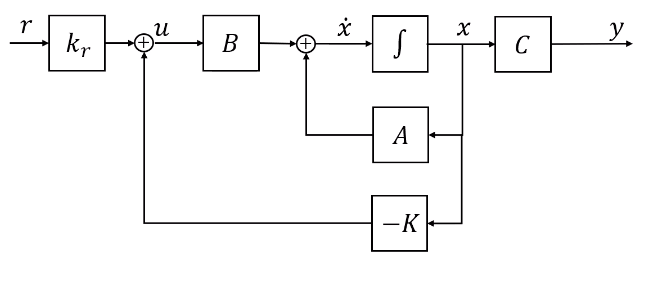
\includegraphics[width=0.6\linewidth]{Bilder/SE_FB_Principle}
	\caption{State-feedback control design principle}
	\label{Fig_SE_SFB_Principle}
\end{figure}

In order to estimate each of the states required by the system given in figure \ref{Fig_SE_SFB_Principle}, the idea of state estimation is to develop an another system called an observer that provides an estimate of dynamical system's states as shown in figure \ref{Fig_SE_Principle}. Further to improve the estimations, a feedback of the original dynamical system's output can be fed into the observer also shown in figure \ref{Fig_SE_Principle}. By using a feedback to the observer, the error dynamics between the observer and dynamical system can be mapped and driven to zero so as to make the estimation more accurate.
\begin{figure}[h!]
	\centering
	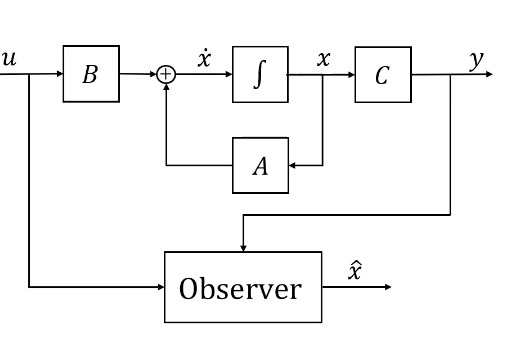
\includegraphics[width=0.6\linewidth]{Bilder/SE_Observer_PRinciple}
	\caption{State estimation principle with observer design}
	\label{Fig_SE_Principle}
\end{figure}

\section{Goal of State estimation}\label{Sec_2_ch_26_goalOfObserver}

Let $\hat{x}$ is the estimated states and $x$ is the actual states, such that the error between them is expressed as,
\begin{equation}
	e = x - \hat{x}
\end{equation}
the error dynamics can be expressed as,
\begin{equation}
	\dot{e} = \dot{x} - \dot{\hat{x}}
\end{equation}

The goal of state estimation can then be formulated as $$ \dot{e} = \dot{x} - \dot{\hat{x}} = 0 $$ the idea is to drive the error between the actual states and the derived states to zero such that we get a replica of the actual states. Such that as $\dot{e} = \dot{x} - \dot{\hat{x}} = 0$, $\hat{x} \rightarrow x$.

In general, the following approach is adopted in order to design a observer and derive required states from it. Consider figure \ref{Fig_GenericObserverDeisgn},
\begin{figure}[h!]
	\centering
	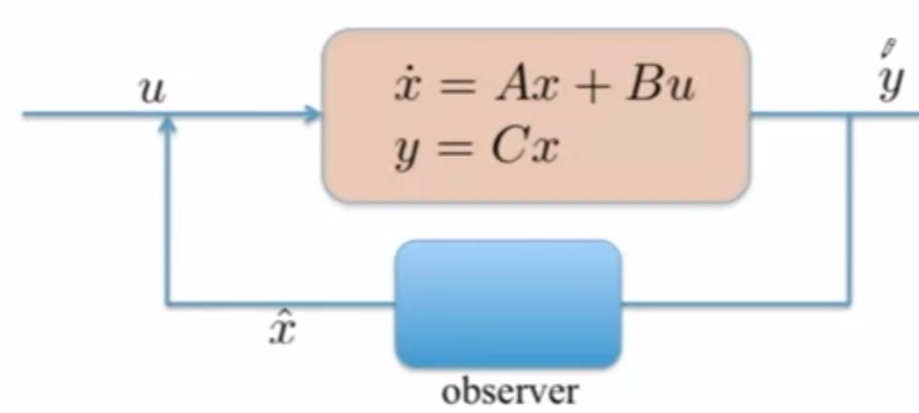
\includegraphics[width=0.5\linewidth]{Bilder/SS4.png}
	\caption{Generic Observer Design}
	\label{Fig_GenericObserverDeisgn}
\end{figure}
Only the outputs from the system can be measured using sensors, the idea is to figure out the actual system states using the sensed system outputs. As shown in figure \ref{Fig_GenericObserverDeisgn}, the outputs of the system is fed into a device, here so called an observer, based on the sensed outputs, system states are derived.

\textbf{\textit{Note: }}If the observer design does not estimate all the required system states, then a new set of sensors has to be added to the system. New sensed outputs will then drive the system to be completely observable as described in \ref{Sec_Observability}.

\section{Observers design}

\subsection{Theory}

Once observability has been established, the idea of state-estimation using an observer design is to use the system inputs and the outputs of the original system to estimate the states of the original system. In essence, the idea is to use the copy of the original linear dynamical system that uses $u$ as well and $y$ from the original system and has its states $\hat{x}$ which estimates the states of the original system as follows
\begin{equation} \label{eq_2_ch_26_ObserverDesign_prototype}
\frac{d \hat{x}}{dt} = F \hat{x} + Gu + Hy
\end{equation}
Lets begin with a simple observer design, starting for only input $u$ as shown in figure \ref{fig_2_ch_26_ObserverDeisgn1}, therefore the observer model is expressed as,
\begin{figure}[h!]
	\centering
	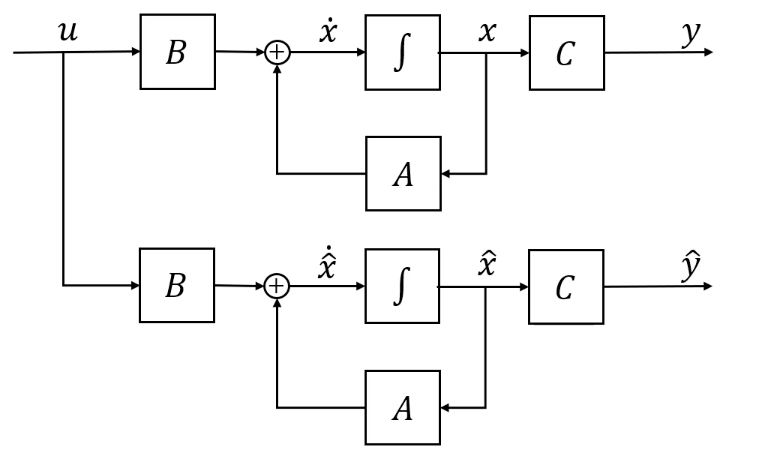
\includegraphics[width=0.6\linewidth]{Bilder/ObserverDesgin1.png}
	\caption{Open-loop observer design}
	\label{fig_2_ch_26_ObserverDeisgn1}
\end{figure}
\begin{equation}
\frac{d \hat{x}}{dt} = A \hat{x} + Bu
\end{equation}
As described in section \ref{Sec_2_ch_26_goalOfObserver}, the goal of an observer is to eliminate the error in the prediction, such that
\begin{equation}
e = x - \hat{x} = 0
\end{equation}
(this error dynamics is also called as \textbf{\textit{Estimator Dynamics}})analyzing error dynamics of this open-loop observer design,
\begin{equation}
\dot{\tilde{x}} = \dot{x} - \dot{\hat{x}} = A {x} + Bu - A \hat{x} - Bu = A {x} - A \hat{x} = A (x - \hat{x}) = A {\tilde{x}}
\end{equation}
from the above equation, it can be seen that the error dynamics of the state estimation is completely dependent on the actual error itself and independent of inputs to the system. In order to determine the behavior of the error dynamics given by the system above, the solution to $\tilde{x}$ has to be found. The system $\dot{\tilde{x}} = A {\tilde{x}}$ is in standard canonical form, the solution to which is expressed as $\tilde{x} = e^{At}\tilde{x}(0) = e^{At}(x(0) - \hat{x}(0))$. This says that the error response will be dependent on the eigenvalues of A as well as the initial conditions. Therefore, if A has eigenvalues in positive half-plane then this open-loop observer design system will be un-stable. Which means that the estimation of states would not be appropriate to be used in most / any of the systems at all.

Now, consider another system with feedback. Because feedback has earlier proven to be effective by shifting the eigenvalues of the system towards the negative half-plane. A closed-loop observer design is employed using output feedback to the observer design as shown in figure \ref{fig_2_ch_26_ObserverDeisgn2}
\begin{figure}[h!]
	\centering
	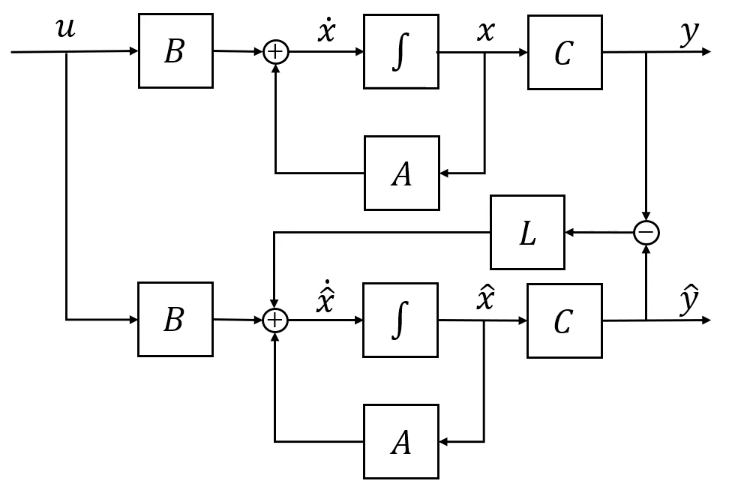
\includegraphics[width=0.6\linewidth]{Bilder/ObserverDesign2.png}
	\caption{Closed-loop observer design}
	\label{fig_2_ch_26_ObserverDeisgn2}
\end{figure}
In case of closed-loop observer design, the estimated output and the measured output are first compared $y - \hat{y}$ and then fed back into the observer design using a feedback gain $L$, so that $L$ can be adjusted to shift the eigenvalues towards the left half-plane. In this case now, the new observer can be modeled using figure \ref{fig_2_ch_26_ObserverDeisgn2} as following
\begin{equation}\label{eq_2_ch_26_ObserverDesign_2}
\dot{\hat{x}} = A \hat{x} + Bu + L (y - \hat{y})
\end{equation}
now the system \eqref{eq_2_ch_26_ObserverDesign_2} is finally appearing to be modeled according to \eqref{eq_2_ch_26_ObserverDesign_prototype}. Further, analyzing error dynamics similar to the open-loop observer design,
\begin{align*}
\dot{\tilde{x}} &= \dot{x} - \dot{\hat{x}} \\
&= A {x} + Bu - A \hat{x} - Bu - L\tilde{y} \\
&= A(x - \hat{x}) - L (y - \hat{y}) \\
&= A(x - \hat{x}) - L (Cx - C\hat{x}) \\
&= A\tilde{x} - LC\tilde{x} \\
&= (A - LC)\tilde{x}
\end{align*}
from the above result, it can be seen that the closed-loop observer design give a possibility to tune the eigenvalues of the system which would otherwise be unstable because of the eigenvalues of A. Further, the response can be determined using the solution of the equation. The system $\dot{\tilde{x}} = (A - LC)\tilde{x}$ is in standard canonical form, the solution to which is expressed as $\tilde{x} = e^{(A-LC)t}(x(0) - \hat{x}(0))$. With the system response given by
\begin{equation}
	y = \vec{C}\hat{x}
\end{equation}

\subsection{State estimation gain}

The way to choose state estimator gain is similar to that used fo control design. Using the closed loop estimator, the error dynamics becomes
\begin{equation}
	\dot{\tilde{x}} = (A - LC)\tilde{x}
\end{equation}

Therefore, now using system \eqref{eq_2_ch_26_ObserverDesign_2} it is now possible to choose feedback gain $L$ such that the error dynamics converges to $\tilde{x} \rightarrow 0$ as $t \rightarrow \infty$, (if observable).

In order to make the error dynamics go to zero, poles of the observer has to be selected such that the error states $\tilde{\dot{x}}$ go to zero. The closed-loop poles for this observer design can be found using,
\begin{equation} \label{Eq_2_ch_26_ObseverGainPoles}
det(s - A + LC) = 0
\end{equation}

\subsection{Predictor-Corrector}

Predictor-Corrector is essentially the same closed-loop observer design only modeled in a different way.

This is one of the simplest observer designs. Consider a system by ignoring the system inputs $Bu$ such that the state dynamics and output be expressed by,
\begin{align}
	\dot{x} &= A x \\
	y &= C x
\end{align}
The observer design is as follows,
\begin{itemize}
	\item Predictor: Make a copy of the system such that the new system has the state dynamics $\dot{\hat{x}} = A \hat{x}$
	\item Corrector: Next add the error between the copy systems output and the output of the actual system. The output of the actual system is given by $y = C x$ and that of copy system is $\hat{y} = C \hat{x}$. Since this is a linear system, the effects of error signal can be directly superimposed into the system as follows,
	\begin{equation}
		\dot{\hat{x}} = A \hat{x} + (y - C \hat{x})
	\end{equation}
	\item Additionally, also add a scaling factor, a gain $L$ so that the error signal $e = (y - C \hat{x})$ can be adjusted, such that it can be driver to zero. Therefore,
		\begin{equation}\label{eq_observerDesign1}
	\dot{\hat{x}} = A \hat{x} + L(y - C \hat{x})
	\end{equation}
	\item The term $e = (y - C \hat{x})$ from \eqref{eq_observerDesign1} is the estimation error, with the goal of driving this error to zero, such that $e = x - \hat{x}$, the idea is to drive the dynamics of error to zero. In this case,
	\begin{equation}\label{Eq_ObserverDesign2}
		\dot{e} = \dot{x} - \dot{\hat{x}} = Ax - A \hat{x} - L(y - C \hat{x})
	\end{equation}
	if $\dot{e}$ needs to be driven to zero, the equation \eqref{Eq_ObserverDesign2} can be stabilized asymptotically such that, the dynamics are driven to zero asymptotically.The only the difference here would be that, in this case, the asymptotic stability will be when the dynamics is towards zero.
	
	Further, simplify \eqref{Eq_ObserverDesign2},
	\begin{equation} \label{Eq_ErrorDynamics}
		\dot{e} = A (x - \hat{x}) - LC (x - \hat{x}) = (A - LC) e
	\end{equation}
	\item It can be seen that using the error dynamics equation \eqref{Eq_ObserverDesign2}, the error of the observer can be directly diminished to zero without even considering the determined states $\hat{x}$.
	\item In the final step, consider the matrix $(A - LC)$ there is only one variable in this matrix, that is $L$, $L$ can be adjusted appropriately by choosing appropriate eigenvalues such that the error dynamics diminish to zero. For the simplest case, a pole placement method can be used.
\end{itemize}

\subsection{Example of observer design}

Consider a system,
\begin{equation}
	\dot{x} = \begin{bmatrix}
		-1 & 2 \\ 0 & -2
	\end{bmatrix} x, \quad y = [1 \quad -1]x
\end{equation}
The error dynamics can be determined using the expression \eqref{Eq_ObserverDesign2}
\begin{equation*}
		\dot{e} = (A - LC) e
\end{equation*}
here $A$ is of size $(2\times2)$, $C$ is of the size $(1\times2)$, therefore, $L$ should be sized to $(2\times1)$ as $[L_{1} \quad L_{2}]^{T}$
\begin{align*}
	\dot{e} &= \left(\begin{bmatrix}
	-1 & 2 \\ 0 & -2
	\end{bmatrix} - \begin{bmatrix}L_{1} \\ L_{2} \end{bmatrix} [1 \quad -1] \right) e \\
			&= \begin{bmatrix}
				-1-L_{1} & 2 + _{1} \\ -L_{2} & -2+L_{2}
			\end{bmatrix} e
\end{align*}
for pole placements, now the characteristic equation \eqref{Eq_StSp_CL_Poles} $sI - (A - LC)$ in this case,
\begin{align*}
	det(sI - (A - LC)) &= det\left(\begin{bmatrix}
	\lambda + 1 + L_{1} & -2-L_{1} \\ L_{2} & \lambda + 2 - L_{2}
	\end{bmatrix} \right) \\
					&= \lambda^{2} + \lambda(3 + L_{1} - L_{2}) + 2 + 2L_{1} + L_{2}
\end{align*}
choosing a characteristic equation $p_{des} = \lambda^{2} + 2 \lambda + 1$ for desired pole placements and matching the coefficients,
\begin{align}
	\lambda(3 + L_{1} - L_{2}) &= 2 \\
	2 + 2L_{1} + L_{2} = 1
\end{align}
$L_1$ and $L_2$ can be determined as,
\begin{align}
	L_1 &= -2 /3 \\
	L_2 &= 1 / 3
\end{align}
Once $L_1$ and $L_2$ have been determined, the determined states dynamics can be determined using
\begin{equation}
	\dot{\hat{x}} = A \hat{x} + \begin{bmatrix}
		-2/3 \\ 1 / 3
	\end{bmatrix} (y - C \hat{x})
\end{equation}

\subsection{Example observer design fo Single Track Model} \label{Sec_2_ch_26_ObserverDesignSingleTrackModel}

Consider a single track model shown below which is modeled as per in section \ref{Sec_2_ch_26_SingleTrackModel},
\begin{equation}
	\begin{bmatrix}
	\dot{x}_{1} \\ \dot{x}_{2}
	\end{bmatrix} = \begin{bmatrix}
	0 & 12 \\ 0 & 0
	\end{bmatrix}\begin{bmatrix}
	{x}_{1} \\ {x}_{2}
	\end{bmatrix} + \begin{bmatrix}
	6 \\ 3
	\end{bmatrix}u
\end{equation}
\begin{equation}
	y = [1 \quad 0] \begin{bmatrix}
	\dot{x}_{1} \\ \dot{x}_{2}
	\end{bmatrix}
\end{equation}
where $x_{1}$ is the lateral position $Y$, $x_2$ is the heading orientation $\theta$ and $u$ is the steering angle $\delta$. The estimator design requirement is to design an observer such that it uses the measurement of vehicles lateral position to estimate vehicle's states. 

The requirement that the observer should stabilize the estimated states earlier than the controller can use them, the poles of the observer are placed at the negative LHP as $\{s_1, s_2\} = \{-6,-4\}$. Therefore, a desired characteristic polynomial can be expressed as
\begin{equation}\label{Eq_2_ch_26_ExObserverDesign2_1}
	p_{des}\lambda = (\lambda + 6)(\lambda + 4) = \lambda^{2} + 10 \lambda + 24
\end{equation}

The closed-loop observer design is chosen as given in \eqref{eq_2_ch_26_ObserverDesign_2} where the estimated states are determined by
\begin{equation}\label{Eq_2_ch_26_ExObserverDesign2_2}
	\dot{\hat{x}} = A \hat{x} + Bu + L (y - \hat{y})
\end{equation}
and the estimator dynamics (error dynamics) are given by the characteristic equation
\begin{equation}
	\tilde{\dot{x}} = (A - LC)\hat{x} = \left( \begin{bmatrix}
	0 & 12 \\ 0 & 0
	\end{bmatrix} - \begin{bmatrix}
	l_1 \\ l_2
	\end{bmatrix} [1 \quad 0]\right) \begin{bmatrix}
	\tilde{x}_{1} \\ \tilde{x}_{2}
	\end{bmatrix}
\end{equation}
here, $C$ is of size $1\times2$, the required size of $LC$ is $2\times2$ therefore, $L$ should be chosen in size $2\times1$

Simplifying, the above equation
\begin{equation}
\tilde{\dot{x}} = \left( \begin{bmatrix}
0 & 12 \\ 0 & 0
\end{bmatrix} - \begin{bmatrix}
l_1 & 0 \\ l_2 & 0
\end{bmatrix}\right)\begin{bmatrix}
\tilde{x}_{1} \\ \tilde{x}_{2}
\end{bmatrix} = \left( \begin{bmatrix}
-l_1 & 12 \\ -l_2 & 0
\end{bmatrix}\right)\begin{bmatrix}
\tilde{x}_{1} \\ \tilde{x}_{2}
\end{bmatrix}
\end{equation}

the poles of this estimator is given by
\begin{equation}
	det(sI - A + LC) = \lambda^2 + l_1 \lambda + 12 l_2
\end{equation}

for the observer design, these poles should match the required polynomial in \eqref{Eq_2_ch_26_ExObserverDesign2_1}
\begin{equation}
	\lambda^{2} + 10 \lambda + 24 = \lambda^2 + l_1 \lambda + 12 l_2 \implies l_1 = 10 \quad l_2 = 2
\end{equation}

Finally, plugging in the values of observer gains into the closed-loop observer,
\begin{equation}
	\dot{\hat{x}} = \begin{bmatrix}
	0 & 12 \\ 0 & 0
	\end{bmatrix}\begin{bmatrix}
	{x}_{1} \\ {x}_{2}
	\end{bmatrix} + \begin{bmatrix}
	6 \\ 3
	\end{bmatrix}u + \begin{bmatrix}
	10 \\ 2
	\end{bmatrix}(y - \hat{x}_{1})
\end{equation}

\subsection{Control using the estimated states}

From the observer gains now determined, estimated states are derived using \eqref{Eq_2_ch_26_ExObserverDesign2_2} and used for the feedback control design $u = -K\hat{x} + k_{r}r$. The control algorithm using the controller itself and the observer as a whole now forms the whole of the controller (developed as software) of the system as shown by the highlighted figure \ref{fig_2_ch_26_ControlUsingEstimatedStates}
\begin{figure}[h!]
	\centering
	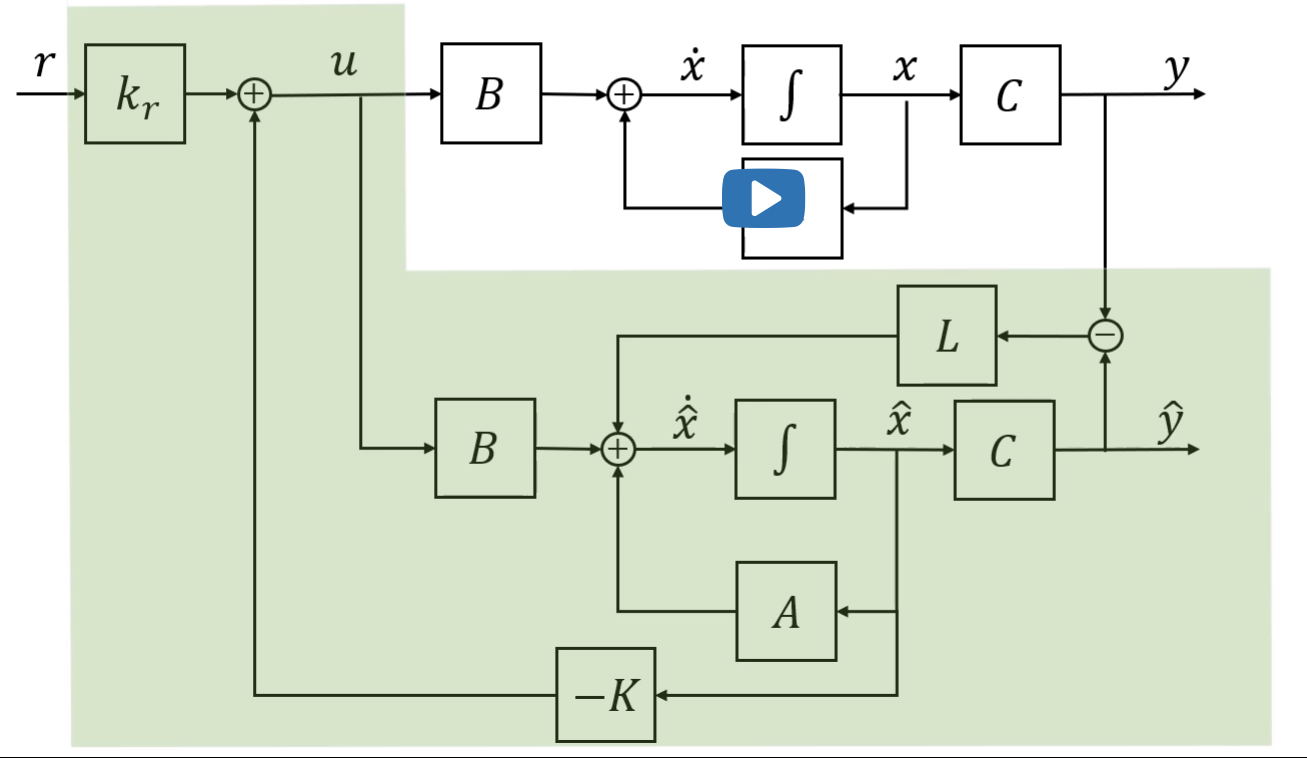
\includegraphics[width=0.75\linewidth]{Bilder/ControlFromEstimatedStates.png}
	\caption{Control algorithm using estimated states}
	\label{fig_2_ch_26_ControlUsingEstimatedStates}
\end{figure}
At this point of system design, now we have a given system $\dot{x} = Ax + Bu$ with output $y = Cx$ and the feedback controller $u = -K\hat{x} + k_{r}r$. Additionally with a state estimator $\hat{\dot{x}} = A \hat{x} + Bu + L (y - C\hat{x})$, for which the eigenvalues are adjusted such that the error dynamics $\tilde{\dot{x}} = (A - LC)\tilde{x}$. The complete closed-loop system can be written as
\begin{equation}\label{Eq_2_ch_26_ControlUsingEstimatedStates_1}
	\begin{bmatrix} \dot{x} \\ \tilde{\dot{x}} \end{bmatrix} = \begin{bmatrix}
	A - BK & BK \\ 0 & A - CL
	\end{bmatrix}\begin{bmatrix}
	x \\ \tilde{x}
	\end{bmatrix}\begin{bmatrix}
	B k_r \\ 0
	\end{bmatrix}
\end{equation}
in \eqref{Eq_2_ch_26_ControlUsingEstimatedStates_1}, the states $x$ are replaced with the estimated states $\hat{x}$. There are two closed-loops in this system with the closed loop poles given by $\lambda(s)$. Each of these closed-loop poles are determined separately and as a system as a whole can be expressed as
\begin{equation}\label{Eq_2_ch_26_ControlUsingEstimatedStates_2}
	\lambda(s) = det(sI - A + BK) \quad det(sI - A +LC)
\end{equation}
provided that this system is both controllable and observable, the polynomial \eqref{Eq_2_ch_26_ControlUsingEstimatedStates_2} can be assigned roots such that the eigenvalues for each of the closed-loop can be adjusted to stabilize the system. In general, the poles of observer are chosen such that they are 4-5 times faster than the poles of feedback controller. As an observer is only a piece of software code and no actuator, the observer cannot be simply saturated with high observer gains. Therefore, this system is practical.

\subsection{Full System with Observer and Feedback controller}

Consider the observer design as describe in section \ref{Sec_2_ch_26_ObserverDesignSingleTrackModel} for a single track vehicle model. For the observer poles placed at $\{s_1, s_2\} = \{-4,-6\}$, the observer gains $\{l_1,l_2\}$ were found to be $\{10,2\}$.

Consider a feedback controller with a double pole placed at $\{s_1,s_2\} = \{-1,-1\}$ for which the controller gains $\{k_1,k_2\} = \{0.0278,0.6111\}$, additionally with the steady-state reference tracking gain $k_r = 0.0278$ therefore the control law can be written as,
\begin{equation}
	u = -Kx + k_r r = -0.0278 x_1 - 0.6111 x_2 + 0.0278 r
\end{equation}

the full system with both the closed loop controller and observer are expressed as,
\begin{equation}
	\dot{\hat{x}} = A \hat{x} + Bu + L(y - C\hat{x}) = \begin{bmatrix}
	0 & 12 \\ 0 & 0
	\end{bmatrix}\begin{bmatrix}
	{x}_{1} \\ {x}_{2}
	\end{bmatrix} + \begin{bmatrix}
	6 \\ 3
	\end{bmatrix}u + \begin{bmatrix}
	10 \\ 2
	\end{bmatrix}(y - \hat{x}_{1})
\end{equation}

\subsection{Implementation - Digital Computer Language}
The system developed so far needs to be transformed into a discrete system before being implemented as a software for the computer. From the system developed in the previous section, the state-estimator can be developed in discrete form using a first order Euler's approximation in this case as
\begin{equation}
	\dot{\hat{x}} \approx \frac{\hat{x}(t_{k+1}) - \hat{x}(t_{k})}{t_{k+1} -t_{k} } = A \hat{x}(t_{k}) + B u(t_{k}) + L(y(t_{k}) - C\hat{x}(t_{k})
\end{equation}
the next state can be derived by rearranging the above equation as
\begin{equation}
	\hat{x}(t_{k+1}) = \hat{x}(t_{k}) + ({t_{k+1} -t_{k} }) \left( A \hat{x}(t_{k}) + B u(t_{k}) + L(y(t_{k}) - C\hat{x}(t_{k}) \right)
\end{equation}
where $({t_{k+1} -t_{k} }) = h$ is the sampling time. In pseudo-code, the control algorithm can be expressed as,
\begin{lstlisting}
	// control algorithm - main loop
	r = digital_read(ch1)	// read reference
	y = diitial_read(ch2)	// read process outputs
	// from previous computed state and r
	u = -K*xhat + k_r*r	// compute control variable
	analog_out(ch1, u)	// set the analog output
	/* (ch1 is the summation point both for reference
	and control variable) */
	xhat = xhat + h*(A*x + B*u + L*(y-C*x))	
	// update next state
\end{lstlisting}

\section{Observability} \label{Sec_Observability}

\textbf{\textit{Definition: }} A linear system is observable if for every $T > 0$, it is possible to determine the state of the system $x(t)$ through the measurements of $y(t)$ and $u(t)$ on the interval of $[0,T]$.

Similar to Controllability not being able to control any arbitrary system, not all systems can also be completely observable. In most of such cases, a rich set of sensor skirt has to be added additionally, such that it improves the output $y$ and from there $\hat{x}$ can be determined.

Consider a modest example of a discrete system with no input as given below, 
\begin{align}
x_{k+1} &= A x_{k} \\
y_{k} &= C x_{k}
\end{align} 
The question is, can the initial state be recovered given $n$ number of outputs, 
\begin{align}
y_{0} &= C x_{0} \\
y_{1} &= C x_{1} = C A x_{0}
\end{align}
iterating this upto $n$ number of outputs, $$y_{n-1} = C A^{n-1} x_{0}$$ writing the above
iteration in matrix form,
\begin{equation}
	\begin{bmatrix}y_{0} \\y_{1} \\ y_{2} \\ . \\ . \\. \\ y_{n-1}
	\end{bmatrix} = \begin{bmatrix}C \\ CA \\ CA^{2} \\ . \\ . \\. \\ C A^{n-1} \end{bmatrix} x_{0}
\end{equation}
here the matrix on the RHS is called the Observability matrix $\Omega$, with the system being observable only when $\Omega$ has a full rank of $n$. If it is the case that with enough number og outputs, the initial states can be tracked that means, that the each of the intermediate states from the current outputs upto the initial states can also be tracked.

\subsection{Observability Theorem 1}

The system is completely observable (CO), if it is possible to recover
the initial state from the output. Therefore, the system is CO iff
$rank(\Omega) = n $

\subsection{Observability Theorem 2}

Pole-placement to arbitrary eigenvalues is possible iff the system is
CO.

***Note:*** With observer design, a close approximation of the states
$\hat{x}$ can be made, all by having only the outputs $y$.

\section{Separation Principle}

So far, in this book most of the fundamental tools have been developed from Controllability, Observability, State feedback, Observers and Pole-Placement technique. In practice for example, pole-placement is a technique used to stabilize the dynamics of both the controller and the observer. However, each of them is dependent on another, a controller needs the observer to estimate the states of the system such that $\hat{x} \approx x$. Only a fairly estimated states by the observer can lead to the controller to work properly as expected. On the other hand, te observer also needs the inputs from the controller for the states estimation. So it appears that there are two dependent systems the inputs of each are dependent on the outputs from the another.

This complication is solved using the Separation principle.

\subsection{Method of separation principle}

Assume a system that is completely controllable and completely observable, given by
\begin{align*}
	\dot{x} &= Ax + Bu \\
	y &= Cx
\end{align*}
the separation principle works in the following steps,
\begin{enumerate}
	\item Design the state feedback controller as if full set of $x$ states were already known (currently which are unknown)
	Using this asumption, the controller can be designed such that
	\begin{equation*}
		u = -K x \implies \dot{x} = (A - BK)x
	\end{equation*}
	As $\hat{x}$ instead of $x$ is known in reality, it is better to use the controller design,
	\begin{equation*}
		u = -K \hat{x} \implies \dot{x} = (A - BK)\hat{x}
	\end{equation*}
	This completes the required control design, now observer design can be proceeded with the observer design
	\item Estimate $x$ using an observer (that now also contains u)
	Previously, in the Predictor-Corrector observer design, $u$ was ignored as in a linear system such external signals can be added at anytime. Consider a system with $u$ inputs,
	\begin{equation*}
		\dot{\hat{x}} = A \hat{x} + B u + L (y - C\hat{x})
	\end{equation*}
	where $A \hat{x} + B u$ is the predictor part and $L (y - C\hat{x})$ is the corrector part of the observer. The error dynamics remains the same as,
	\begin{equation*}
		\dot{e} = (A - LC) e
	\end{equation*}
	\item The dynamics of both $x$ and $e$ needs to be stabilized, therefore in the separation principle both $\dot{x}$ and $\dot{e}$ are considered together for analyzing the dynamics as,
	\begin{equation}\label{Eq_2_ch_9_rand1}
		\dot{x} = Ax - BK \hat{x} = Ax - BK (x - e) = (A - BK)x + BKe
	\end{equation}
	here, as the controller is always designed for the estimated sates $\hat{x}$, therefore in \eqref{Eq_2_ch_9_rand1} $Bu = - K \hat{x}$. Also, using he relationship $e = (x - \hat{x})$, \eqref{Eq_2_ch_9_rand1} is replaced with $e$ so as to write the following equations.
	\begin{equation}\label{Eq_2_ch_9_rand2}
		\begin{bmatrix}
		\dot{x} \\ \dot{e}
		\end{bmatrix} = \begin{bmatrix}
			A - BK & BK \\ 0 & A - LC
		\end{bmatrix} \begin{bmatrix}
			x \\ e
		\end{bmatrix}
	\end{equation}
	The strategy of separation principle works if an only if, \eqref{Eq_2_ch_9_rand2} is an asymptotically stable system.
	Observe, that the matrix in the RHS of \eqref{Eq_2_ch_9_rand2} is a upper triangular block matrix, with the blocks of matrices $A - BK$ and $A - LC$ along the diagonals. In such a triangular block matrix, the eigenvalues of the entire matrix are simply the eigenvalues of the diagonal blocks. Such that, if this whole triangular matrix is represented by $m$, then
	\begin{equation}
		det(m) = det(A - BK) det(A - LC)
	\end{equation}
\end{enumerate}

\subsection{Choosing eigenvalues for controller and observer}

In general, as the controller is dependent on the correct prediction of the observer to correctly control the system as desired, it is always should be the case that the observer poles are placed such that the slowest pole of the observer is always much faster than the controller poles. For example, the poles are arbitrarily placed as shown in figure \ref{fig_2_ch_9_polesofControllerAndObserver}
\begin{figure}[h!]
	\centering
	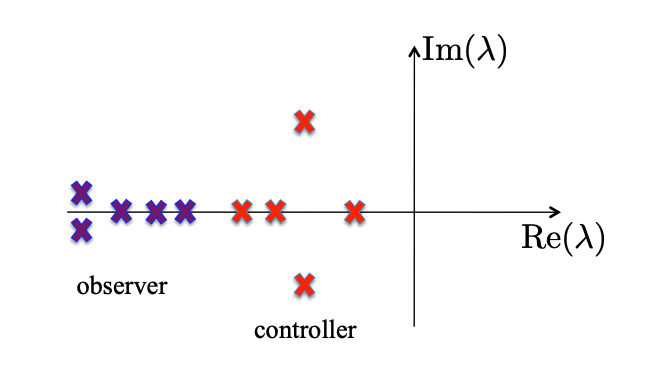
\includegraphics[width=0.65\linewidth]{Bilder/SS5.png}
	\caption{Poles of controller and observer}
	\label{fig_2_ch_9_polesofControllerAndObserver}
\end{figure}

\section{Kalman Filter}

Consider again the linear time invariant system which is added with process disturbances and measurement noise given by:
\begin{align}
	\dot{x} &= Ax + Bu + v \\
	y &= Cx + w
\end{align}
where $v$ and $w$ are stochastically added process disturbances and measurement noise, included into the system so as to define the use of a filter. Earlier, a feedback observer design was used which had the state estimator dynamics as \eqref{eq_2_ch_26_ObserverDesign_2}
\begin{equation}
	\dot{\hat{x}} = A\hat{x} + Bu + L(y - C\hat{x})
\end{equation}
as now the process disturbances and measurement noise are included into the system, the error $\tilde{x} = x - \hat{x}$ will be effected by these parameters and the error dynamics can be determined using the the equation
\begin{equation}
	\dot{\tilde{x}} = \dot{x} - \dot{\hat{x}}
\end{equation}
substituting for $\dot{x}$ and $y$ from the equations stated above, the following equation is derived
\begin{align*}
	\dot{\tilde{x}} &= Ax + Bu + v - A\hat{x} - Bu - L(Cx + w - C\hat{x}) \\
					&= Ax + v - A\hat{x} - L(Cx + w - C\hat{x}) \\
					&= Ax - A\hat{x} - LC(x - \hat{x}) + v - Lw \\
					&= A\tilde{x} - LC\tilde{x} + v - Lw \\
					&= (A - LC)\tilde{x} + v - Lw 
\end{align*}
From the above expression it can be seen that the error dynamics is characterized by the system matrix $(A - LC)$, therefore, if $(A - LC)$ is stable, then the estimation error becomes stable. In this case, since a stochastic process is included into the system, the error here becomes \textbf{\textit{stationary stochastic process}}. Using covariance, the error can be linearly transformed using $P_{\tilde{x}}$ = $\mathbb{E}(\tilde{x}(t)\tilde{x}^{T}(t))$, using this formulation, the covariance of the estimation error is given by the following equation
\begin{equation}
	0 = (A - LC)P_{\tilde{x}} + P_{\tilde{x}}(A - LC)^{T} + R_{v} + L R_{w}L^{T}
\end{equation}
the idea here is to minimize the covariance matrix ($P_{\tilde{x}}$) using matrix $L$. The optimal observer therefore, minimizes $P_{\tilde{x}}$.

***Note*** If the system is time-varying, the system will also be time dependent.

\subsubsection{Kalman - Bucy Filter}

Kalman - Bucy discovered that when the system is observable, the optimal observer gain matrix $L$ is given by
\begin{equation}
	L = P_{\tilde{x}} C^{T} R_{w}^{-1}
\end{equation}
where $P_{\tilde{x}} = P^{T}_{\tilde{x}} \geq 0$ is the solution to the Riccati equation
\begin{equation}
	0 = A P_{\tilde{x}} + P_{\tilde{x}} A^{T} + R_{v} - P_{\tilde{x}}C^{T}R_{w}L^{-1}CP_{\tilde{x}}
\end{equation}
This observer is called the \textbf{\textit{Kalman - Bucy Filter}} which has the following characteristics
\begin{itemize}
	\item always stable
	\item the optimal linear filter for state estimation
	\item  $R_{v}$ and $R_{w}$ are regarded as the design parameters. $R_{v}$ can be decided using the sensor characteristics.
\end{itemize}
There are similarities between Kalman Filter and LQR, in-fact, using them both in the controller design \textbf{\textit{linear quadratic Gaussian controller}}.

\subsection{Vehicle Steering Example}

Consider the steering model which is modeled as per in section \ref{Sec_2_ch_26_SingleTrackModel}, added with stochastic processes $v$ and $w$
\begin{equation}
\begin{bmatrix}
\dot{x}_{1} \\ \dot{x}_{2}
\end{bmatrix} = \begin{bmatrix}
0 & 12 \\ 0 & 0
\end{bmatrix}\begin{bmatrix}
{x}_{1} \\ {x}_{2}
\end{bmatrix} + \begin{bmatrix}
6 \\ 3
\end{bmatrix}u + \begin{bmatrix}
v_{1} \\ v_{2}
\end{bmatrix}
\end{equation}
\begin{equation}
y = [1 \quad 0] \begin{bmatrix}
\dot{x}_{1} \\ \dot{x}_{2}
\end{bmatrix} + w
\end{equation}

The process disturbance and the measurement noise are zero mean with covariance (linear transformation of disturbances)
\begin{align}
	R_{v} &= \begin{bmatrix}
	1 \quad 0 \\ 0 \quad 1
	\end{bmatrix} \\
	R_{w} &= \rho
\end{align}
The idea is to design a Kalman filter to estimate the vehicles states, from the measurement of the lateral position. The standard state estimator equation is used ($\dot{\hat{x}} = A\hat{x} + Bu + L(y - C\hat{x})$) with $L$ as the optimal observer gain given by the Kalman filter equation $L = P_{\tilde{x}} C^{T} R_{w}^{-1}$. Where $P_{\tilde{x}} = P^{T}_{\tilde{x}} \geq 0$ is the solution to the Riccati equation
\begin{equation}
0 = A P_{\tilde{x}} + P_{\tilde{x}} A^{T} + R_{v} - P_{\tilde{x}}C^{T}R_{w}L^{-1}CP_{\tilde{x}}
\end{equation}
and, the solution to the Riccati equation is given by (for example)
\begin{equation}
	\begin{bmatrix}
	p_{1} \quad p_{2} \\ p_{2} \quad p_{3}
	\end{bmatrix}
\end{equation}
inserting the solution $P_{\tilde{x}}$ into the Riccati equation gives a non-linear matrix equality
\begin{equation}
	\begin{bmatrix}
	0 \quad 0 \\ 0 \quad 0
	\end{bmatrix} = \begin{bmatrix}
	0 \quad 12 \\ 0 \quad 0
	\end{bmatrix} \begin{bmatrix}
	p_{1} \quad p_{2} \\ p_{2} \quad p_{3}
	\end{bmatrix} + \begin{bmatrix}
	p_{1} \quad p_{2} \\ p_{2} \quad p_{3}
	\end{bmatrix} \begin{bmatrix}
	0 \quad 0 \\ 12 \quad 0
	\end{bmatrix} + \begin{bmatrix}
	1 \quad 0 \\ 0 \quad 1
	\end{bmatrix} + \rho^{-1} \begin{bmatrix}
	p_{1} \quad p_{2} \\ p_{2} \quad p_{3}
	\end{bmatrix} \begin{bmatrix}
	1 \\ 0
	\end{bmatrix} [1 \quad 0] \begin{bmatrix}
	p_{1} \quad p_{2} \\ p_{2} \quad p_{3}
	\end{bmatrix}
\end{equation} 
this Riccati equation can be solved using Matlab \textbf{[P,E,L] = care(A',C',[[1 \quad 0]; [0 \quad 1]], 1)}, choosing noise covariance of $\rho = 1$, gives the following result
$$P_{\tilde{x}} = \begin{bmatrix}
5.0 \quad 1.0 \\ 1.0 \quad 0.4167
\end{bmatrix}$$ and
$$\begin{bmatrix}
5.0 \\ 1.0
\end{bmatrix}$$

\subsection{Kalman Filter Matrix Equations}

The design of Kalman filter has five matrices as described below:
\begin{enumerate}
	\item $\vec{x}$ the state matrix
	\item $\vec{P}$ the uncertainty matrix. This is of size $(n \times n)$ where $n$ is the number of states. This matrix says about how confident we are when the states prediction is concerned by the filter. The higher the number the higher uncertainty is when states prediction is concerned. In case of Kalman filter, this is the only tuner that will be available to tune the filter to make better predictions. Only elements along the diagonals of this matrix are tuned.
	\item $\vec{F}$ the state transition matrix. This is of size $(n \times n)$ where $n$ is the number of states. This matrix is same as the $A$ matrix in linear state-space equation 
	\item $\vec{H}$ the measurement matrix. This is of size $(z \times n)$ where $z$ is the number of sensors. This matrix gives a relationship that is required to extract measured states such as velocity from the speed-o-meter. In most of the simple cases the  $\vec{H}$ has 1's along its diagonal indicating a one-to-one relationship between measurement and the states. This matrix is similar to $C$ matrix in the linear state space equation.
	\item $\vec{R}$ the measurement uncertainty matrix. This is of size $(n \times n)$. This matrix has to say about the certainty of the measurements recorded. If the measurements recorded can be claimed to be 100$\%$ accurate, then the corresponding terms in this matrix can be made zero. The values are plugged only along the diagonal and the weighted values are determined through trail and error until a suitable solution is converged.  
\end{enumerate}

Once these matrices have been established, then a computation method is employed in order to perform the \textbf{\textit{Predictions}} and \textbf{\textit{Measurements and Update}}. Both predictions and measurements and update computations are central to all of the filters. The part in the measurements and update (state update for the next time-integration) will be employed specifically for specific type of a filter such as a Kalman Filter. 

Using the five matrices generated, the following computations are performed:
\begin{enumerate}
	\item \textbf{\textit{Predictions}}
	\begin{enumerate}
		\item $x = \vec{F} x$
		\item $\vec{P} = \vec{F}\vec{P}\vec{F}^{T} $
	\end{enumerate}
	\item \textbf{\textit{Measurements and Update}}
	\begin{enumerate}
		\item $\vec{Z} = $measurements
		\item $y = \vec{Z}^{T} - \vec{H}x$
		\item $\vec{S} = \vec{H}\vec{P}\vec{H}^{T} + \vec{R}$
		\item $\vec{K} = \vec{P}\vec{H}^{T}\vec{S}^{-1}$
		\item $x = x + \vec{K}y$
		\item $\vec{P} = (\vec{I} - \vec{K}\vec{H})\vec{P}$
	\end{enumerate}
\end{enumerate} 







